\documentclass[a4paper,10pt]{article}
\usepackage[utf8]{inputenc}
\usepackage[MeX]{polski}
\usepackage{graphicx}

\title{[MBI.A] Asembler DNA, sparowane końce - dokumentacja końcowa}
\author{Michał Aniserowicz, Jakub Turek}
\date{}

\begin{document}

\maketitle

\section*{Opis problemu}

Zadanie polega na implementacji aplikacji, która umożliwia tworzenie \emph{scaffoldów} na podstawie dostarczonych zbiorów \emph{contigów} oraz sekwencji PET. 

\begin{center}
  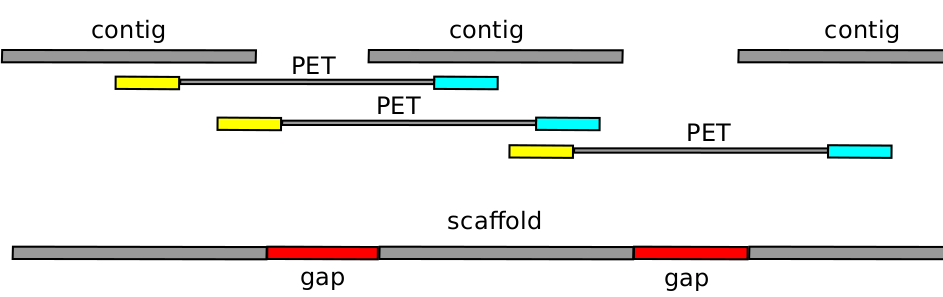
\includegraphics[width=.9\textwidth]{contig_pet.png}
\end{center}

\section*{Założenia}

W~ogólnym przypadku rekonstrukcja sekwencji \emph{contigów} nie jest możliwa. Z~tego względu, na potrzeby projektu przyjęto następujące założenia:

\begin{itemize}
  \item Początki i~końce łańcuchów PET to sekwencje unikalne. Wystąpienie takiej sekwencji w~jednym z~\emph{contigów} oznacza, że jest to odpowiednio początek lub koniec sekwencji PET.
  \item Badane są wyłącznie takie permutacje \emph{contigów}, dla których wystąpienie początku sekwencji PET implikuje przynajmniej częściowe wystąpienie jej końca w~dalszej części łańcucha. Innymi słowy początek lub koniec sekwencji PET nie może w~całości wystąpić w~przerwie (\emph{gap}) \emph{scaffoldu}.
  
    \begin{itemize}
	  \item Wyjątkiem od tej reguły jest początek i~koniec \emph{scaffoldu}, gdzie mogą występować, odpowiednio, niesparowane końce lub początki sekwencji PET.
    \end{itemize}
  
  \item Sekwencje należące do różnych par sparowanych końców mogą częściowo zachodzić na siebie.
\end{itemize}

\section*{Algorytm}

Do rozwiązania zadania użyty został algorytm typu brute-force działający na wstępnie odfiltrowanym zbiorze kombinacji contigów.
Algorytm przebiega według następującego schematu:

\begin{enumerate}
 \item Wyznaczane są wszystkie permutacje zadanego zbioru \emph{contigów}.
 \item Permutacjie zostają wstępnie sprawdzone:
  \begin{itemize}
   \item następuje próba znalezienia sekwecji PET, której początek i koniec w całości zawiera się w dowolnej parze \emph{contigów}:
    \begin{itemize}
     \item jeśli taka sekwencja nie zostanie znaleziona, wszyskie permutacje zostają uwzględnione w kolejnych krokach algorytmu;
    \end{itemize}
   \item każda permutacja jest sprawdzana pod względem kolejności wystąpienia \emph{contigów} zawierających znalezioną sekwencję:
    \begin{itemize}
     \item jeśli \emph{contig} zawierający początek sekwencji znajduje się przed \emph{contigiem} zawierającym jej koniec, to dana permutacja zostaje uwzględniona w kolejnych krokach algorytmu,
     \item w przeciwnym wypadku, permutacja zostaje odrzucona.
    \end{itemize}
  \end{itemize}
 \item Na podstawie każdej z zaakceptowanych permutacji budowany jest \emph{scaffold}:
  \begin{itemize}
   \item dla każdej sekwencji PET:
    \begin{itemize}
     \item następuje próba znalezienia \emph{contiga} zawierającego (w całości lub częściowo\footnote{Częściowe zawieranie sekwencji PET występuje, gdy \emph{contig} zaczyna się końcem fragmentu (tzn. początku lub końca) danej sekwencji lub kończy początkiem fragmentu tej sekwecji.}) początek sekwencji,
     \item przeglądane są \emph{contigi} występujące po znalezionym, w celu odnalezienia \emph{contiga} zawierającego koniec sekwecji,
     \item jeśli odległość pomiędzy znalezioną parą \emph{conitgów} dopuszcza istnienie pomiędzy nimi sekwencji PET, to  pomiędzy te \emph{contigi} wstawiany jest odpowiedniej długości \emph{gap},
     \item jeśli w którymkolwiek z powyższych kroków nastąpiło niepowodzenie (odpowiedni \emph{conitg} nie został odnaleziony lub sprawdzenie odległości dało wynik negatywny), to wykonywane jest sprawdzenie, czy pierwszy \emph{contig} zawiera koniec sekwecji lub czy ostatni \emph{conitg} zawiera jej  początek - taka sytuacja uznawana jest za poprawną,
     \item aktualizowany jest ranking \emph{R}, określający liczbę pokrywających się zasad początku lub końca sekwencji PET z odnalezionymi \emph{contigami}.
    \end{itemize}
   \item jeżeli \emph{R} $> 0$, to dany \emph{scaffold} dodawany jest listy wynikowej algorytmu.
  \end{itemize}
 \item Uzyskana lista \emph{scaffoldów} sortowana jest według malejących wartości \emph{R}.
\end{enumerate}

\section*{Implementacja}

Projekt został zaimplementowany w~języku C\# (platforma .NET). Testy jednostkowe zostały napisane w~oparciu o~platformę NUnit\footnote{http://www.nunit.org/}, z~użyciem biblioteki Rhino Mocks\footnote{http://www.ayende.com/wiki/Rhino+Mocks.ashx}.

Aplikacja posiada interfejs okienkowy stworzony w~technologii WPF, umożliwiający odczyt danych wejściowych z/zapis danych wyjściowych do pliku. Na dane wejściowe składają się:

\begin{itemize}
 \item Opis \emph{conitgów} w~postaci łańcuchów tekstowych oddzielonych znakami nowej linii.
 
  \begin{verbatim}
    ACAGCTTA
    CCGGGTAC
    TACAGCTT
  \end{verbatim}
  \item Opis sekwencji PET w~postaci dwóch sekwencji (początek, koniec) oraz długości łańcucha. Dane w~sekwencji oddzielone przecinkami, natomiast kolejne PET'y oddzielone znakami nowej linii.
  
  \begin{verbatim}
   GATC,CCAT,100
   GGCT,AGAA,1500
  \end{verbatim}
\end{itemize}

Dane wyjściowe to uporządkowana sekwencja \emph{contigów} oddzielonych znakami spacji reprezentującymi długość przerwy (\emph{gap}).

  \begin{verbatim}
   CCGGGTAC       TACAGCTT  ACAGCTTA
  \end{verbatim}

\section*{Przykład}

\begin{itemize}
 \item Plik wejściowy:
  \begin{verbatim}
   ACAGCTTA
   CCGGGTAC
   TACAGCAA

   CCG,TACA,15
   GCA,GCT,13
  \end{verbatim}
 \item Plik wyjściowy:
  \begin{verbatim}
   CCGGGTAC   TACAGCAA   ACAGCTTA
  \end{verbatim}
\end{itemize}

\section*{Testowanie}
TODO

\end{document}